\chapter{Fiber bundles}\index{Bundle}

In the language of modern geometry, fiber bundles serve as a unifying framework, extending classical notions such as vector bundles to a broader setting. They naturally arise in various mathematical and physical contexts, providing a structural backbone for spaces with local product structures.

\,
A principal application appears in Gauge Theory, where principal bundles furnish a natural setting for describing gauge fields in physics, including the Yang-Mills theories. Here, the connection on a bundle encodes the dynamics of fundamental interactions, and curvature expresses field strength in a geometrically intrinsic way.

\, 
In topology, fiber bundles play a fundamental role in the theory of characteristic classes, such as the Chern classes, which assign global topological invariants to vector bundles. These invariants capture deep global properties of manifolds, serving as indispensable tools in the study of topology, geometry, and mathematical physics.

\, 
\section{Definitions and examples}

The notion of bundle have been introduced to generalize topological product.

\begin{definition}[Fiber bundle]\index{Bundle!Fiber bundle}
A fiber bundle is a triple $(\cB,\cM,\pi)$ consisting of two topological spaces
$\cB$ and $\cM$ and a continuous surjective map
\[
\pi:\cB \to \cM,
\]
where $\pi$ is called the projection of the total space $\cB$ onto the base space $\cM$.
\end{definition}

\vspace{3pt}
The topological space $\cF_{\scriptstyle M}= \pi^{-1}({\scriptstyle M}), \, {\scriptstyle M}\in \cM$
 is called the fibre at ${\scriptstyle M}\in \cM$.

\

\begin{example}
The simplest example of bundle is the product bundle defined by $(E_{1}\times E_{2},E_{1},\pi) $ where $E_{i}$ is isomorphic to $\bbR$ and with $\pi(x,y)=x$, for all $x \in E_{1}$ and $y\in E_{2}$. This is illustrated by the following diagram.

\begin{center}
    \begin{tikzpicture}[scale=0.7]
    % Draw axes (orthogonal frame)
    \draw[thick,->] (0,0) -- (5,0) node[below right] {$E_1$};
    \draw[thick,->] (0,0) -- (0,4) node[above left] {$E_2$};
    % Draw quadrant label
    \node at (1.3,1.5) { $E_1 \times E_2$};
    % Draw point (x,y)
    \filldraw (3,2) circle (2pt);
    \node[above right] at (3,2) { $(x,y)$};
    % Draw projection onto x-axis
    \draw[dashed,->] (3,2) -- (3,0.3);
   % \draw[dashed] (3,0.3) -- (3,0);
    \filldraw (3,0) circle (2pt);
    \node[below] at (3,0) {$(x,0)$};
    % Label for projection
    \node at (3.5,1) { $\pi$};
\end{tikzpicture}
\end{center}

So, in this example the total space is given by the topological product $\cB= E_1 \times E_2$ and the base space is $\cM=E_1 $. The projection map is given by $\pi(x,y)=x$, where we project $E_1 \times E_2$ onto $ E_1$. Naturally, we could have chosen to project on $E_2$. 
\end{example}

\,

The need to generalize topological products can be seen on the following examples.
 

a) The cylinder is obtained by taking the topological product $S^{1}\times \mathcal{I}$, where $\mathcal{I}$ is  a segment. The fiber bundle is defined by the triple $(S^{1}\times \mathcal{I},S^{1},\pi)$, where here we have chosen to define the projection map as follows $\pi:S^{1}\times \mathcal{I} \to S^1$ .

\begin{center}
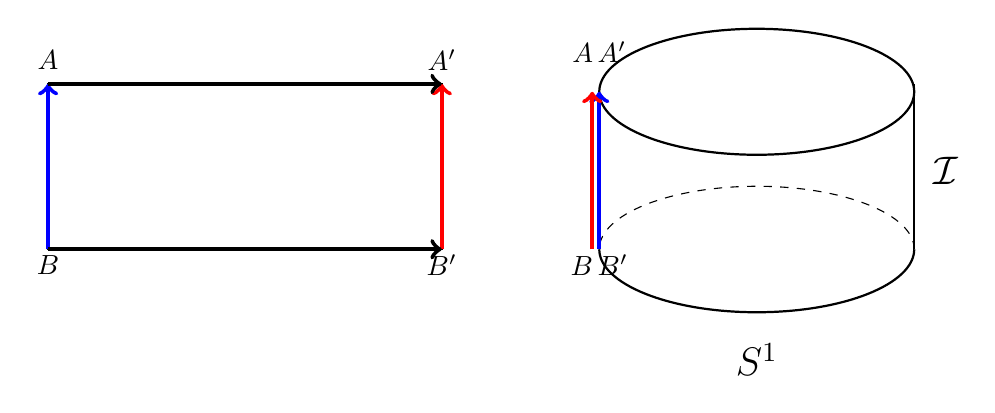
\begin{tikzpicture} 
     \draw[thick] (-9,0) rectangle (-4,2.1);
         \draw[ultra thick,blue, ->] (-9,0) -- (-9,2.1);
    \draw[ultra thick,red, ->] (-4,0) -- (-4,2.1);
   \draw[ultra thick,black, ->] (-9,0) -- (-4,0);
    \draw[ultra thick, black, ->] (-9,2.1) -- (-4,2.1);
     \node at (-9,-0.2) { $B$}; 
       \node at (-4,-0.2) { $B'$}; 
  \node at (-9,2.4) { $A$};
   \node at (-4,2.4) { $A'$}; 

  \draw[dashed] (2,0) arc[start angle=0,end angle=180,x radius=2cm, y radius=0.8cm];

    \draw[thick] (2,0) arc[start angle=0,end angle=-180,x radius=2cm, y radius=0.8cm];

    \draw[thick] (0,2) ellipse (2cm and 0.8cm);   
      \draw[ultra thick,blue,->] (-2,0) -- (-2,2);
     \draw[ultra thick,red,->] (-2.09,0) -- (-2.09,2);
    \draw[thick] (2,0) -- (2,2.1);
    % Labels
    \node at (0,-1.4) {\Large $S^1$};   
      \node at (2.4,1) {\Large $\mathcal{I}$}; 
 \node at (-2.0,-0.2) { $B\, B'$}; 
  \node at (-2,2.5 ) { $A\, A'$}; 
\end{tikzpicture}
\end{center}


\,


b) The M\"obius band obtained by twisting a sheet and then gluing the opposite edges forms only a local topological product and is {\it no longer a topological product}. It can be done locally: for an open subset $U\subset S^1$, the topological product $U \times \cI$ describes a segment of the  M\"obius band, but does not take under account  the twisting operation.

\begin{figure}[h]
\includegraphics[scale=0.6]{Mobius_3.pdf}
  \hspace{0.3cm}\includegraphics[scale=0.25]{Mobius_2.pdf}
 \end{figure}

\,

\subsection{Properties}
In the following we restrict ourselves to the case  where the topological space $\cF_{\scriptstyle M}= \pi^{-1}({\scriptstyle M}), \, {\scriptstyle M}\in \cM$ are  homeomorphic to a space $F$, called typical fibre.


\begin{definition}[Trivial bundle]\index{Bundle!Trivial bundle}
A trivial bundle $\cB$ is a fiber bundle homeomorphic to a product bundle $\cM\times \cF$ and
$ \pi $ is just the projection from the product space to $\cM$.
\end{definition}



\begin{definition}[Vector bundle]\index{Bundle!Vector bundle}	
	\noindent If $\cF_M$ is a vector space, $(\cB,\cM,\pi)$ is  called vector bundle.
\end{definition}

\begin{definition}[G-bundle]\index{Bundle!G-bundle}
A fiber bundle $(\cB,\cM,\pi, G)$ is  made of:
\begin{enumerate}
	\item a bundle $(\cB,\cM,\pi)$
together with a typical fiber $\cF$, 

\vspace{3pt}
	\item a topological group $G$ of homeomorphisms of $\cF$ onto itself (called the structural group)
	
	\vspace{3pt}
	\item a covering by open sets $\{U_j\}_{j\in J \subseteq \bbN}$ where  $U_j \in\cM$  such that:

\vspace{3pt}
\begin{enumerate}
\item Locally, the bundle is a trivial bundle.

\vspace{3pt}
\item Let ${\scriptstyle M}\in U_i\cap U_j$, the homeomorphism $ {\psi_{\scriptscriptstyle M}}_i\circ {\psi_{\scriptscriptstyle M}}_{j}^{-1}: \cF \to\cF$, where
${\psi_{\scriptscriptstyle M}}_{i}$ denote a homeomorphism from $\cF_x$ onto $\cF$, is an element of the structural group $G$ for all $i,j \in J$.

\vspace{3pt}
\item The induced mapping $\gamma_{ij}: U_i\cap U_j \to G$ by $\gamma_{ij}(x)=  {\psi_{\scriptscriptstyle M}}_i\circ {\psi_{\scriptscriptstyle M}}_{j}^{-1}$ is continuous.
\end{enumerate}
\end{enumerate}
\end{definition}

\begin{definition}[Principal fiber bundle]\index{Bundle!Principal fiber bundle}
A $G$-bundle $(\cB,\cM,\pi, G)$ in which the typical fiber $\cF$ and the structural groupe $G$ are isomorphic by left translation~\footnote{Let $G$ be a group the action \[L_{g}:G\to G \text{ by } L_{g}(h)=gh\] is called left translation.} is called a principal fiber bundle.
\end{definition}


\begin{definition}[Vector bundle]\index{Bundle!Vector bundle}	
	\noindent If $\cF$ is a vector space, $(\cB,\cM,\pi)$ is  called vector bundle.	
\end{definition}
A vector bundle is a $G$-bundle with $G$ the linear group of $\cF$.

\begin{definition}[Cross-section of a bundle] \index{Bundle!Cross-section}
A cross-section of the bundle $(\cB,\cM,\pi,G)$ is a mapping $\sigma: \cB  \to
\cM$ such that $\sigma \circ \pi = I_\cM$ the identity in $\cM$.
\end{definition}

\begin{theorem}
 A principal fiber bundle $(\cB,\cM,\pi, G)$ is trivial if and only if it is a continuous cross-section.
\end{theorem}

\begin{proof}
First assume that $\cB$ has a cross-section $\sigma: \cM \to \cB$. Then
\[
\pi \sigma(x) =x \text{ for } x\in \cB. 
\]
Given $p\in \cF$, there exists a unique $g_0$ such that $p= L_{g_0}=g_0\sigma(x)$. 
Then, 
\[
 \phi_\sigma : \cB \times G \text{ by } p\mapsto (x,g_0)
 \]
 is a homomorphism which preserves the group structure of the fibers
\[ 
\phi_\sigma(L_{g'} p) =L_{g'}\phi(p) \quad \forall g'\in G, \forall p\in \cB.
\]
In particular, $\phi_\sigma(f(x)=(x,e)$, where $e$ is the identity of $G$.
This shows that the existence of a continuous cross-section implies the triviality.

Conversely, if the principal bundle is trivial i.e. $\cB= \cM \times G$,  then \[f:\cM \to \cM \times G\] defined by $x\mapsto (x,k(x))$ (where $k : X \to G$ is some continuous mapping) forms a cross-section of $\cB$.
\end{proof}

\subsection{Tangent bundles and frame bundles} The notion of tangent spaces can be upgraded to the structure of a tangent bundle. We describe this in the next section below. 
\subsection{\bf Tangent bundle}
\begin{definition}[Tangent  bundle] \index{Bundle!Tangent bundle}
A tangent bundle $(\cT(\cM),\cM,\pi,G)$ is a bundle with fibers being the tangent spaces. 
\end{definition}

In the case of a $n$-dimensional manifold, the tangent-bundle  $(\cT(\cM), \cM, \pi,G)$ can be identified to the natural bundle defined by
\begin{itemize}
	\item a fiber at ${\scriptstyle M}\in \cM$, $\cF_{{\scriptstyle M}}= \cT_{\scriptstyle M}(\cM)$ and typical fiber $\bbR^{n}$,
	\item a projection $\pi:({\scriptstyle M},X_{{\scriptstyle M}}) \mapsto {\scriptstyle M}$, 
		\item the structural group $G=GL(n,\bbR)$ of linear automorphisms on
$\bbR^{n}$.
\end{itemize}

\subsection{Frame bundle}
Let $\cM$ a $n$-dimensional manifold. A frame $\phi_{\scriptscriptstyle M}$ associated with the tangent bundle $\cT_{\scriptstyle M}(\cM)$ of $\cM$ is a set of $n$ linearly independent vectors $\{f_{1},\dots,f_{n}\}$ which can be expressed as a linear combination of a particular basis  $\{e_{1},\dots,e_{n}\}$ of  $\cT_{\scriptstyle M}(\cM)$, such that 
\[f_{i}=a_{i}^{j}e_{j},\quad \text{for}\quad a \in GL(n,\bbR)\quad \text{and}\quad i\in \{1,\cdots, n\}. \]
This implies that there exists a bijection between the set of all frames in  $\cT_{\scriptstyle M}(\cM)$ and the group $GL(n,\bbR)$.

\begin{definition}[Frame bundle]
Let us consider the collection \[\Phi(\cM)=\{({\scriptstyle M},\phi_{\scriptscriptstyle M}),\, {\scriptstyle M}\in \cM\}\] and $\cM$ is equipped with a differentiable structure. Then, the four-tuple 

$(\Phi(\cM),\cM,\pi, GL(n,\bbR))$ 
with typical fiber $GL(n,\bbR)$ and structural group $GL(n,\bbR)$ is called the frame bundle on $\cM$.
\end{definition}

\, 

Furthermore, a frame bundle associated with a vector bundle 
forms  a principal $GL(n,\bbK)$-bundle, where $\bbK$ is a field of characteristic 0 such as $\bbR$ or $\bbC$. The general linear group acts freely and transitively on the frames via basis changes. 

\, 

The topology on the fiber bundle associated to a vector bundle $E$
 is constructed using local trivializations of 
$E$. Each trivialization induces a bijection between the fiber over 
an open set $U_i$ and $U_i\times GL(n,\bbK)$, with the final topology ensuring compatibility across overlapping regions.
The fibers of the frame bundle are $GL(n,\bbK)$-torsors. A \emph{torsor} (or  principal homogeneous space) for a Lie group $G$ is a homogeneous space for $G$ in which the stabilizer subgroup of every point is trivial. A principal homogeneous space for a group $G$ is a non-empty set on which $G$ acts freely and transitively. 

\, 
\begin{ex}
Prove that when $\cM$ is equipped with a Riemannian metric the  structure group reduces to the orthogonal group 
$O(n)$.  
\end{ex}

\begin{ex}
Prove that when $\cM$ is a $2n$-dimensional symplectic manifold then it has a natural 
$Sp(2n,\bbR)$-structure.  
\end{ex}

We remark the following fact, relating the manifold structure and the frame bundle. 

A natural manifold structure can be given if we  notice that the open sets of the typical fiber  $GL(n,\mathbb{R})$ are in bijection with the open sets of $\bbR^{n^{2}}$, and that the structural group of diffeomorphisms  of the typical fiber onto itself is simply $GL(n,\bbR)$.

\section{Vector fields, Tangent bundles, Lie algebras}
Given a differentiable manifold 
$\cM$, we consider at each point ${\scriptstyle M}$ of $\cM$ its corresponding tangent space $\cT_{\scriptstyle M}(\cM)$. A vector field 
$X$  assigns to every  point in ${\scriptstyle M}\in \cM$ a tangent vector $X_{\scriptstyle M}\in \cT_\cM$ in a smooth manner. This means that if $f$ is a smooth function on $
\cM$, the map 
$p\mapsto X_{\scriptstyle M}(f)$ must also be smooth.
 
In more concrete words, given a subset of the Euclidean space $\bbR^n$, a vector field is represented by a vector-valued function. 

\, 

More fundamentally, a smooth vector field $X$ is a linear map  $X:C^{\infty}(\cM)\to C^{\infty}(\cM)$ where $C^{\infty}(\cM)$ is the algebra of smooth functions and where $X$ satisfies the Leibnitz rule. This property reveals the deep algebraic nature of vector fields: they form a Lie algebra under the Lie bracket, defined as
\[[X,Y](f)=X(Y(f))-Y(X(f)),\] with $f\in C^{\infty}(\cM)$ and $X,Y$ are smooth vector fields on $\cM$.

\, 

To make a link between the previous section on tangent bundle, let us highlight that a vector field on $\cM$ can be defined in terms of a section of the tangent bundle. This is stated in a more precise way in the following definition.

\, 


\begin{definition}[Vector field]\index{Vector field}
A vector field $X$ on a manifold $\cM$ is a cross-section of the tangent bundle
$\cT(\cM)$.
\end{definition}
Using this approach, we can say that a vector field $X$ associates to each ${\scriptstyle M} \in \cM$ a tangent vector $ X_{\scriptstyle M} \in T_{\scriptstyle M}(\cM)$ by the mapping $X: {\scriptstyle M} \mapsto ({\scriptstyle M}, X_{\scriptstyle M})$.


A vector field $X \in \cT(\cM)$ act on differentiable function $f$ on $\cM$ by
\begin{equation}
(Xf)({\scriptstyle M}) =X_{\scriptstyle M} (f), 
 \end{equation}
or in local coordinates,
\begin{equation}~\label{E:tgvecfield}
X=\sum_{i=1}^n X^i\,\frac{\partial}{\partial x^i},  \quad X^{i}=X(\varphi^{i})
\end{equation}
where $X^i$ are functions such that in a chart $(\cU,\varphi)$ in the neighborhood of $M$ by $ X_{\scriptstyle M}^{i}=(X(\varphi))({\scriptstyle M})$, is called the component of
$X$ with respect to the local coordinates $x^i=\varphi^{i}({\scriptstyle M})$. 

\begin{definition}[$\cC^{r}$-vector field]
By definition, a vector field on a $\cC^{k}$-manifold $\cM$ is  $\cC^{r}$-differentiable if the mapping $\cM \to T(\cM)$ is $\cC^{r}$-differentiable, where $r\leq k-1.$
\end{definition}


Going back to out first definition, we can refine it for $\cC^{k}$-differentiable functions of a vector field $X$ on a $\cC^{k}$-manifold $\cM$, can be understood as a derivation on the algebra $\cC^{k}(\cM)$ of function of class $\cC^{k}$ on $\cM$:
\[X: \cC^{k}(\cM)\to \cC^{k}(\cM),\]
\[X(f)({\scriptstyle M})=(Xf)({\scriptstyle M}) \text{ denoted } X(f)=Xf. \]


\subsection{Vector field Lie algebra}\index{Lie algebra}
Let us introduce the space $\fT(\cM)$ of all $\cC^{\infty}$ vectors fields on $\cM$, that is the space of all  $ X(f)$ which are differentiable for all
$\cC^{\infty}$ functions $f$ on $\cM$ . 
Under the addition and the multiplication operation:
\[(X+Y)(f)=X(f)+Y(f),\quad X,Y \in \fT(\cM),\, f \in \cC^{\infty}(\cM), \] 
\[gX(f)=g\big(X(f)\big),  X \in \fT(\cM),\, f,g  \in \cC^{\infty}(\cM) \]
this forms a module on the ring \footnote{A ring is a set $\fR$ with two internal  laws, addition and multiplication. For the addition $\fR$ is an abelian group, the multiplication is associative and distributive with respect to addition.
\[ (xy)z=x(yz),\quad x(y+z)=xy+xz,\quad (y+z)x=yx+zx,\quad \forall x,y,z\in\fT.\]

A module $\fT$ over the ring $\fR$ is an abelian group together with an external operation, called scalar multiplication such that
\[ \alpha(x+y)=\alpha x+\alpha y, \quad (\alpha+\beta)x=\alpha x+\beta x,\quad  (\alpha\beta)x= \alpha (\beta x ),  \quad x,y\in\fT,\,\alpha,\beta \in\fR.
\] } $C^{\infty}(\cM)$, but cannot be an algebra for the product of vector fields. 

The product $XY$ of two vector fields defined by $(XY)(f)=X(Y(f))$ does not satisfy the Leibnitz rule. Indeed, 
\[\begin{aligned}
(XY)(fg)&=X(Y(fg))=X\big(fY(g)+gY(f)\big)\\&=X(f)Y(g)+ fX(Y(g))+X(g)Y(f)+gX(Y(f))\\&\not=f(XY(g))+g(XY(f))=g(X(Y(f))+f(X(Y(g)).
\end{aligned}\]
Therefore $XY$ does not form a vector field.

However, notice that the Lie bracket \index{Lie algebra!Lie bracket} $[\cdot,\cdot]$ defined by
   \begin{equation}
[X,Y]f= X(Y(f))-Y(X(f)),\quad X,Y\in \fT,
 \end{equation}
does form a vector field. The multiplication, defined by the lie bracket is :

\begin{itemize}
\item distributive with respect to the addition,
\item anti-commutative,
\item not associative but satisfies the Jacobi identity: \index{Lie algebra!Jacobi's identity}
 \begin{equation}
[[X,Y],Z]+[[Y,Z],X]+[[Z,X],Y]=0,\quad X,Y,Z\in \fT,
 \end{equation}
 \end{itemize}
 
 \begin{lemma}
  The set $\fT(\cM)$ is a Lie algebra~\footnote{ A Lie algebra is a module  with bracket as internal product.} for the Lie bracket.
\end{lemma} 
\begin{proof}
The proof is mostly described above. \end{proof}

 \begin{definition}[Moving Frame]\label{D:Movfram}\index{Bundle!moving frame}
 A set of $n$ linearly independent differentiable vector fields $\{e_{i}\}_{i=1}^{n }$ which form a basis of the module $ \fT(U)$ where $U\subset \cM$ is called a moving frame.
 \end{definition}
 
Notice that a moving frame may not exist {\it globally} on $T(\cM)$.


To end this section, let us mention that vector fields can be used for instance in Index Theory. The Poincaré--Hopf theorem relates zeros of vector fields on $\cM$ to the Euler characteristic of $\cM$. 

\section{Cotangent bundle - Covector field}
The topic considered in this section relates to cotangent bundles. A cotangent bundle is the natural dual to the tangent bundle, encoding the differential structures of a manifold in their most intrinsic form. While the tangent bundle $\cT(\cM)$ describes directions of motion, the cotangent bundle 
$\cT^*(\cM)$  is the realm of differentials. 

For a differentiable manifold $\cM$  the cotangent space at each point consists of linear functionals on the tangent space. That is, if $X_{\scriptstyle M}$ is a tangent vector, an element of $\cT_{\scriptstyle M}^*(\cM)$ assigns to it a real number by evaluating a differential:
\[df_{\scriptstyle M}(X_{\scriptstyle M}).\]
\subsection{Cotangent bundle}

\begin{definition}[Cotangent bundle]\index{Bundle!Cotangent bundle}
The bundle space $(\cT^\star(\cM),\cM,\pi)$ where $\cT^\star(\cM)$ is the space of pairs
$({\scriptstyle M},\omega_{\scriptstyle M})$ for all ${\scriptstyle M}\in \cM$ and all $\omega_{\scriptstyle M}\in \cT^\star_{\scriptstyle M}(\cM)$ is called
cotangent bundle space. 
\end{definition}

In the case of a n-dimensional manifold,
the cotangent-bundle  $(\cT^{\star}(\cM), \cM, \pi,G)$ can be identified to the natural bundle
\begin{itemize}
	\item  fiber at ${\scriptstyle M} \in \cM$, $\cF_{\scriptstyle M}= \cT^{\star}_{\scriptstyle M}(\cM)$ and typical
fiber $\cF =\bbR^n$,  

	\item projection $\pi : ({\scriptstyle M},\omega_{\scriptstyle M}) \mapsto {\scriptstyle M} $, 
		
	\item The structural group $G=GL(n,\bbR)$,   of linear automorphisms on
$\bbR^n$.
\end{itemize}

\subsection{Covector field}
\begin{definition}[Covector field]\index{Covector field}
 A $\cC^k$-differentiable 1-form $\omega$ is a $\cC^k$-cross section of the cotangent bundle. It is often called a covariant vector field.
\end{definition}

A covariant vector field $\omega$ associates to each $ {\scriptstyle M}\in \cM$ a covariant vector $\omega_{\scriptstyle M} \in X\in \cT^{\star}_{\scriptstyle M}(\cM)$ by the mapping \[\omega: {\scriptstyle M}\mapsto ({\scriptstyle M},\omega_{\scriptstyle M}).\]

The covector field $\omega \in  \cT^{\star}(\cM)$ acts on the vector field $X\in  T(\cM)$
by
\begin{equation}
\omega(X)({\scriptstyle M})=\omega_{\scriptstyle M}(X_{\scriptstyle M}).
\end{equation}


If we denote by $ \{dx^{i}\}_{i=1}^{n}$ the dual basis of the  natural basis $\{\partial_{i}=\partial/\partial x^{i}\}_{i=1}^{n}$,
\[dx^{i}\big(\partial_{j}\big) = \partial_{j}\big(dx^{i}\big)=\delta^{i}_{j},\]
and
\[
\omega_{\scriptstyle M}(X_{\scriptstyle M})={\omega_{\scriptstyle M}}_{i} X_{\scriptstyle M}^{i},\quad \omega_{\scriptstyle M}={\omega_{\scriptstyle M} }_{i}\,dx^{i}|_{\scriptstyle M},\quad  X_{\scriptstyle M} =X_{\scriptstyle M}^{i}\, \partial_{i}|_{\scriptstyle M}, \]
where the index ${\scriptstyle M}\in \cM$. 
\, 

From the equation~\eqref{E:difcoord}, we can define the differential 1-form field by:
\begin{equation}
(df(X))({\scriptstyle M})=df|_{\scriptstyle M}(X_{\scriptstyle M}).
\end{equation}
In the natural basis 
\[df=\frac{\partial f}{\partial x^{i}}\,dx^{i},\]
and in an arbitrary local basis  $\{e_{i}\}_{i=1}^{n}$ in $\cT_{\scriptstyle M}(\cM)$, where $\{\varepsilon_{i}\}_{i=1}^{n}$ is the dual basis, it implies that we have: 
\[(df(X))({\scriptstyle M})= X^{i}_{\scriptstyle M} e_{i}|_{\scriptstyle M} (f)= e_{i}|_{\scriptstyle M}(f)\varepsilon^{i}|_{\scriptstyle M}(X_{\scriptstyle M}),\]
and finally
\begin{equation} \label{E:diffieldcoord}
df= e_{i}(f)\varepsilon^{i}.
\end{equation}

\section{Action of a diffeomorphism}\index{Diffeomorphism}

\subsection{Image of a vector field under a diffeomorphism}\index{Diffeomorphism! Image of a vector field}
Assume $\cM$ and $\cM'$ are two manifolds. Let: \[f:\cM\to \cM'\] be a differentiable mapping between  $\cM$ and $\cM'$, such that ${\scriptstyle M}\in \cM$ is mapped to ${\scriptstyle M'}=f({\scriptstyle M})\in \cM'$. 

The map $f$ induces a linear (Jacobian) mapping~\footnote {the Jacobian mapping is sometimes denoted $f'$.} denoted $f_{\star}$, between the tangent space  $T_{\scriptstyle M}(\cM)$ at ${\scriptstyle M}$ and the tangent space $T_{\scriptstyle M'}(\cM')$ at ${\scriptstyle M'}=f({\scriptstyle M})$, 
 \[
  f_{\star} : X_{\scriptstyle M}\mapsto f_{\star}(X_{\scriptstyle M})=X'_{f({\scriptstyle M})},
  \]
   defined in the following way.
   
 Let $g$ a differentiable function in the neighborhood of $f({\scriptstyle M})$. Then, we obtain:  
 
 \begin{equation}\label{E:fstar}
[(f_{\star}(X)(g)](f({\scriptstyle M}))= [X(g\circ f)]({\scriptstyle M}) =X_{\scriptstyle M} (g\circ f)
\end{equation}
\begin{theorem}
Let $f:\cM \to \cM'$ be a $C^\infty$ diffeomorphism between two $n$-dimensional differentiable manifolds. Then $f_{\star}$ is an isomorphism of the Lie algebra: $$ \fT(\cM)\to\fT(\cM),$$ given by 
\begin{equation}
f_{\star}([X,Y])=[f_{\star}(X),f_{\star}(Y)].
\end{equation}
\end{theorem}

\begin{proof}
Exercise!
\end{proof}


\begin{definition}[Invariant vector field]\index{Vector field!Invariant vector field}
A vector field $X$ on $\cM$ is said to be invariant under the diffeomorphism \[f:\cM \to\cM\] if
\begin{equation}\label{E:invecfield}
f_{\star}(X_{\scriptstyle M})=X_{f({\scriptstyle M})},\quad \forall\, {\scriptstyle M}\in \cM.
\end{equation}
\end{definition}

\subsection{Image of a cotangent vector field under a diffeomorphism}\index{Diffeomorphism!Image of a covector field}
Let $\omega_x\in  T^{\star}_x(\cM)$ and $\omega'_{\scriptstyle M'}$ be such that
\[
\omega_{\scriptstyle M} (X_{\scriptstyle M})= \omega'_{\scriptstyle M'}(X'_{\scriptstyle M'}),
\]
The pull-back (reciprocal image) $f^{\star}: \cT^{\star}_{\scriptstyle M'}(\cM') \to \cT^{\star}_{\scriptstyle M} (\cM)$ of a covariant vector $\omega'_{\scriptstyle M'}$ under the differentiable mapping $f$ is defined by the equality:

\begin{equation}
\left(f^{\star}(\omega'_{\scriptstyle M})\right)_{\scriptstyle M}(X_{\scriptstyle M})=\omega'_{\scriptstyle M'}\left(f_{\star}(X)\right |_{\scriptstyle M'}.
\end{equation}

Therefore, the pull-back\index{Diffeomorphism!Pull-back} $f^\star:  T^{\star}(\cM') \to T^{\star}(\cM)$ of the 1-form $\omega'$ under a differentiable mapping $f$ is defined by
\begin{equation}
\left(f^{\star}(\omega')\right)(X)=\omega'\left(f_{\star}(X)\right)\circ f.
\end{equation}

\begin{remark}
The expression of the reciprocal image of a 1-form does not involve $f^{-1}$, whereas it is the case for a vector field.
\end{remark}

\subsection{Tensor field} We generalise the discussion in the previous chapter about tensors. This notion also can evolve using the concept of fiber bundles. 

\, 

In particular, a fiber bundle where the base space is the manifold $\cM$ and the fiber is identified with $\otimes^{p}T^{\star}_{\scriptstyle M}(\cM)\otimes^{q}T_{\scriptstyle M}(\cM)$  at all ${\scriptstyle M}\in \cM$ is called a $(p,q)$-\emph{tensor bundle}.

Notice that a tangent bundle is a $(0,1)$-tensor bundle and that the cotangent bundle is a $(1,0)$-tensor bundle.

\begin{definition}
A $(p,q)$-tensor field on a $C^{k}$-manifold is a $C^{r}$ cross-section, where $r\leq k-1$ of the $(p,q)$-tensor bundle.
\end{definition}

Operations defined in section~\ref{S:tensor} for tensors at a point, are carried over fiber-wise allowing to define similar operations on tensor fields. 

Under these operations, the set of all  $(p,q)$-tensor fields of class  $\cC^{r}$ is a \emph{ module on the ring} $\cC^{r}(\cM)$.



